\documentclass{standalone}
\usepackage{pgfplots}
\pgfplotsset{compat=newest}

\begin{document}
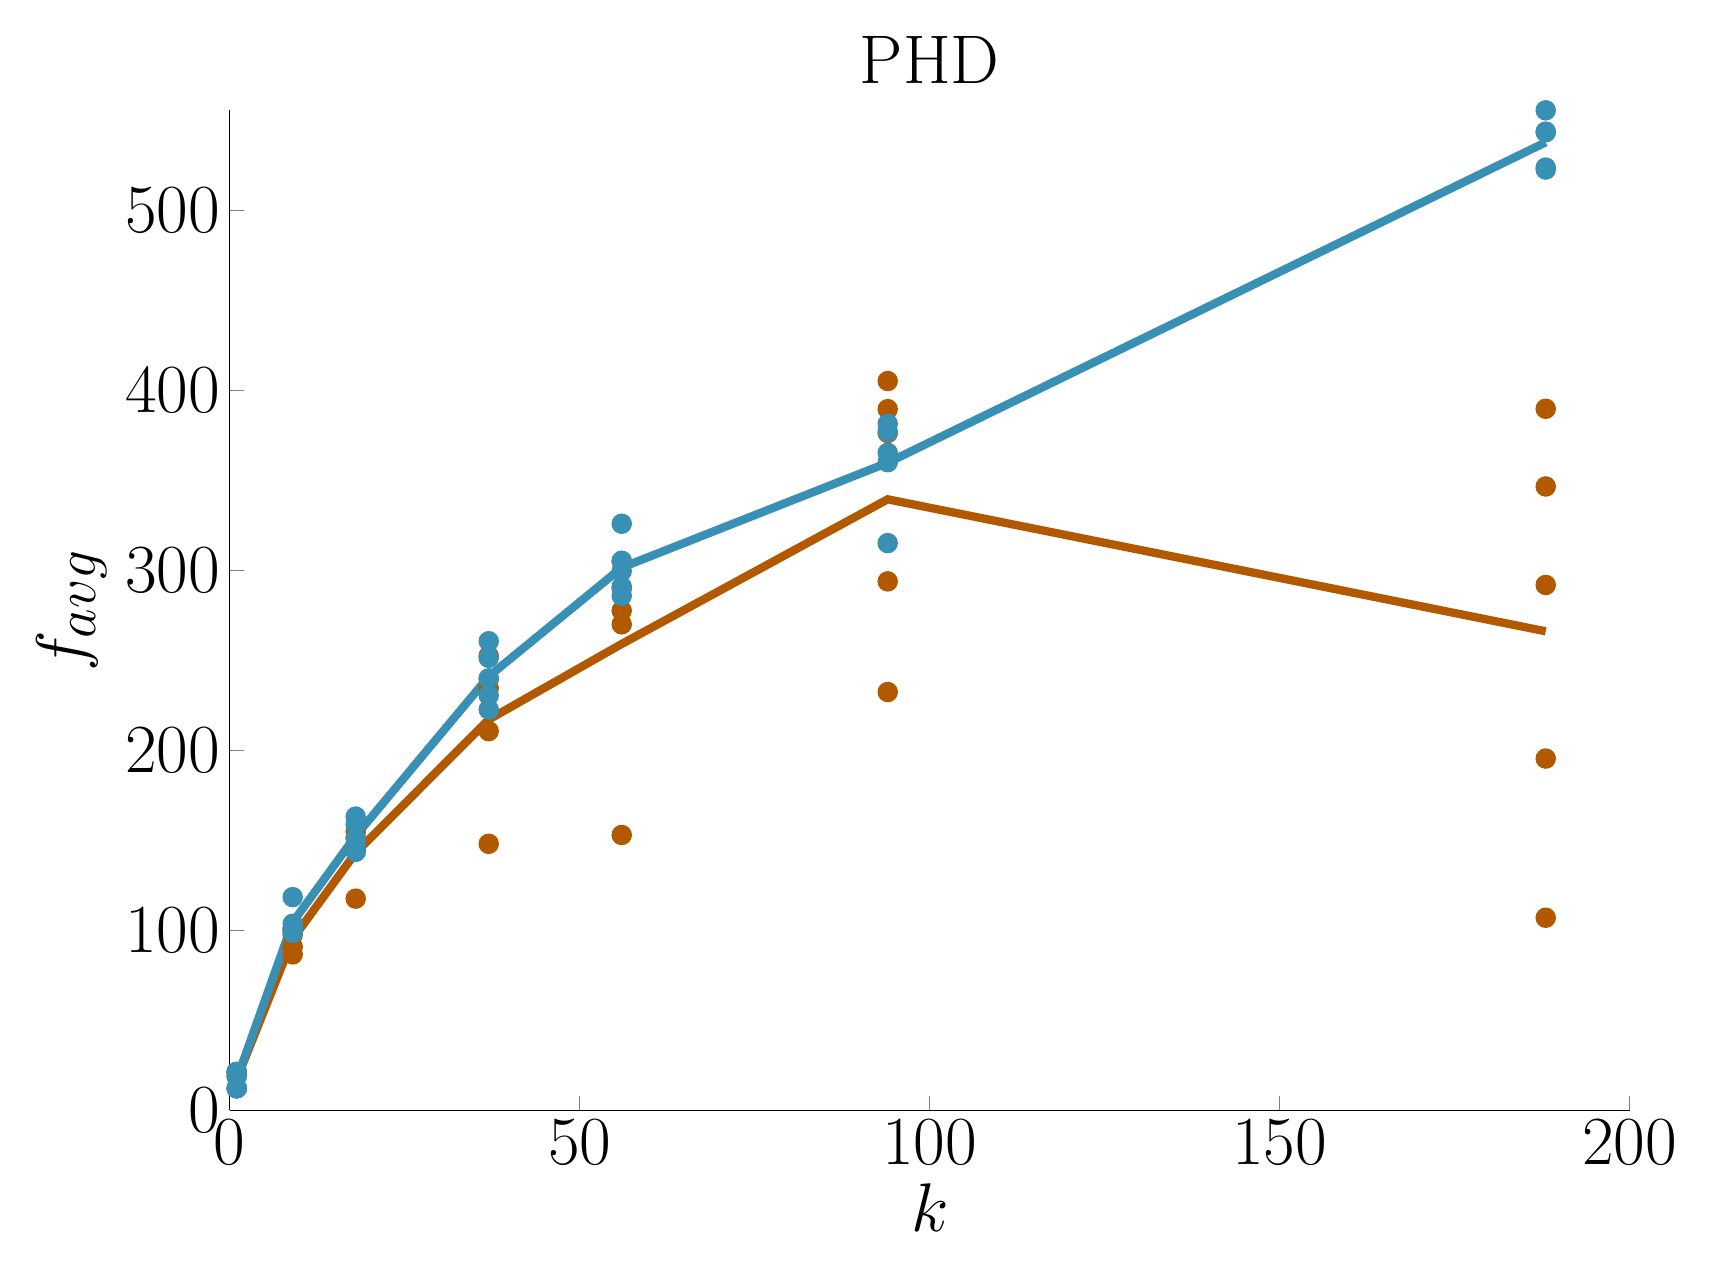
\begin{tikzpicture}

\begin{axis}[%
title style={font=\Huge},
title=PHD,
tick label style={font=\Huge},
label style={font=\Huge},
legend style={font=\Huge},
view={0}{90},
max space between ticks=50pt,
width=7in,
height=5in,
scale only axis,
xmin=0, xmax=200,
xtick={0, 50, 100, 150, 200},
xlabel={$k$},
ymin=0, ymax=555.35,
%ytick={0, 200, 400, 600, 800, 1000},
ylabel={$f_{avg}$},
major tick length=5pt,
axis lines*=left,
legend cell align=left,
clip=false]

\addplot [
only marks,
mark=*,
mark size=3.5pt,
color=orange!70!black,
%solid,
%line width=2pt,
]
coordinates{
(1,12.25)(1,12.25)(1,19.0)(1,21.25)(1,21.25)(9,86.6)(9,90.8)(9,97.4)(9,100.0)(9,101.1)(18,117.55)(18,143.85)(18,147.75)(18,151.4)(18,154.65)(37,148.0)(37,210.55)(37,234.5)(37,239.55)(37,252.35)(56,152.9)(56,269.9)(56,277.5)(56,289.8)(56,304.85)(94,232.3)(94,293.75)(94,376.15)(94,389.4)(94,405.0)(188,106.95)(188,195.35)(188,291.75)(188,346.45)(188,389.6)
};

\addplot [
only marks,
mark=*,
mark size=3.5pt,
color=cyan!70!black,
%solid,
%line width=2pt,
]
coordinates{
(1,12.25)(1,12.25)(1,19.0)(1,21.25)(1,21.25)(9,98.55)(9,100.55)(9,100.85)(9,103.6)(9,118.4)(18,143.55)(18,146.0)(18,150.8)(18,158.75)(18,163.1)(37,222.6)(37,230.4)(37,239.9)(37,251.25)(37,260.5)(56,285.75)(56,290.85)(56,299.45)(56,305.2)(56,325.75)(94,315.0)(94,359.9)(94,365.15)(94,376.85)(94,381.3)(188,522.45)(188,523.55)(188,543.15)(188,543.5)(188,555.35)
};

\addplot [
color=orange!70!black,
solid,
line width=3pt
]
coordinates{
(1,17.2)(9,95.18)(18,143.04)(37,216.99)(56,258.99)(94,339.32)(188,266.02)
};

\addplot [
color=cyan!70!black,
solid,
line width=3pt
]
coordinates{
(1,17.2)(9,104.39)(18,152.44)(37,240.93)(56,301.4)(94,359.64)(188,537.6)
};


\end{axis}
\end{tikzpicture}
\end{document}
